\chapter{Практическая часть}
\section{Текст программы}
\lstset{language=matlab}

В листинге~\ref{lst:programm} приведён текст программы.
\begin{lstlisting}[caption={Текст программы},label={lst:programm}]
function lab2()
    X=[
        -2.79, -3.01, -4.07, -2.85, -2.43, -3.20, ...
        -3.72, -4.27, -5.48, -2.38, -4.69, -4.34, ...
        -5.08, -5.01, -4.08, -4.20, -4.74, -1.88, ...
        -3.25, -2.78, -3.56, -3.54, -3.79, -3.18, ...
        -5.08, -4.30, -2.86, -2.45, -3.08, -3.22, ...
        -2.76, -3.20, -3.33, -4.91, -4.06, -3.81, ...
        -3.96, -3.65, -3.77, -4.60, -5.21, -2.67, ...
        -1.95, -2.43, -1.73, -2.50, -3.96, -3.75, ...
        -2.70, -4.26, -3.42, -4.07, -4.74, -3.00, ...
        -4.37, -5.42, -5.00, -4.08, -2.46, -4.33, ...
        -4.08, -3.72, -4.09, -2.96, -3.71, -1.51, ...
        -3.70, -6.48, -4.26, -4.39, -3.16, -4.63, ...
        -2.66, -2.22, -4.79, -2.46, -3.69, -3.35, ...
        -2.32, -4.17, -3.85, -4.93, -2.05, -3.15, ...
        -3.49, -5.70, -2.53, -3.85, -4.32, -3.37, ...
        -3.98, -3.74, -5.28, -2.56, -3.21, -3.10, ...
        -3.78, -3.36, -3.32, -2.59, -2.45, -3.34, ...
        -3.20, -4.14, -4.00, -4.79, -4.02, -4.58, ...
        -4.45, -3.69, -4.53, -3.98, -4.51, -4.44, ...
        -3.78, -4.24, -4.00, -2.46, -2.58, -4.04, ...
    ];

    % Уровень доверия
    gamma = 0.9;
    alpha = (1 + gamma) / 2;
    % Объем выборки 
    n = length(X);
    % Оценка матожидания
    mu = mean(X);
    % Оценка дисперсии
    D = var(X);
    
    % Границы доверительного интервала для матожидания
    [mu_low, mu_high] = borders_mu(n, mu, D, alpha);
    % Границы доверительного интервала для дисперсии
    [var_low, var_high] = borders_var(n, D, gamma);
    
    fprintf('Mean = %.4f\n', mu);
    fprintf('Variance = %.4f\n', D);
    fprintf('Mean in (%.4f, %.4f)\n', mu_low, mu_high);
    fprintf('Variance in (%.4f, %.4f)\n', var_low, var_high);
    
    % Создание массивов точечных оценок и границ доверительных интервалов
    mu_arr = zeros(1, n);
    var_arr = zeros(1, n);
    mu_low_arr = zeros(1, n);
    mu_high_arr = zeros(1, n);
    var_low_arr = zeros(1, n);
    var_high_arr = zeros(1, n);
    
    % Заполнение созданных массивов
    for i = 1 : n
        mu = mean(X(1:i));
        D = var(X(1:i));
        % Точечная оценка матожидания
        mu_arr(i) = mu;
        % Точечная оценка дисперсии
        var_arr(i) = D;

        [mu_low_arr(i), mu_high_arr(i)] = borders_mu(i, mu, D, alpha);
        [var_low_arr(i), var_high_arr(i)] = borders_var(i, D, gamma);
    end
    
    % Построение графиков
    z_mu = (zeros(1, n) + mu);
    plot(10 : n, [z_mu(10:end)', mu_arr(10:end)', mu_low_arr(10:end)', ...
        mu_high_arr(10:end)']);
    xlim([10, n]);
    xlabel('n');
    ylabel('y');
    legend('$\hat \mu(\vec x_N)$', '$\hat \mu(\vec x_n)$', ...
        '$\underline{\mu}(\vec x_n)$', '$\overline{\mu}(\vec x_n)$', ...
        'Interpreter', 'latex', 'FontSize', 18);
    figure;
    z_D = (zeros(1, n) + D);
    plot(10 : n, [z_D(10:end)', var_arr(10:end)', var_low_arr(10:end)', ...
        var_high_arr(10:end)']);
    xlim([10, n]);
    xlabel('n');
    ylabel('z');
    legend('$\hat S^2(\vec x_N)$', '$\hat S^2(\vec x_n)$', ...
        '$\underline{\sigma}^2(\vec x_n)$', '$\overline{\sigma}^2(\vec x_n)$', ...
        'Interpreter', 'latex', 'FontSize', 18);
end

% Функция поиска границ доверительного интервала для матожидания
function [low_border, high_border] = borders_mu(n, mu, D, alpha)
    low_border = mu - sqrt(D) * tinv(alpha, n - 1) / sqrt(n);
    high_border = mu + sqrt(D) * tinv(alpha, n - 1) / sqrt(n);
end

% Функция поиска границ доверительного интервала для дисперсси
function [low_border, high_border] = borders_var(n, D, gamma)
    low_border = ((n - 1) * D) / chi2inv((1 + gamma) / 2, n - 1);
    high_border = ((n - 1) * D) / chi2inv((1 - gamma) / 2, n - 1);
end
\end{lstlisting}

\section{Результат}

В листинге~\ref{lst:result} приведён результат выполнения описанной программы.
\begin{lstlisting}[language=,numbers=none,caption={Результат программы},label={lst:result}]
Mean = -3.6762
Variance = 0.8664
Mean in (-3.8170, -3.5353)
Variance in (0.7088, 1.0875)
\end{lstlisting}

На рисунке \ref{img:plot01} представлен график оценки математического ожидания.
\begin{figure}[H]
    \centering
    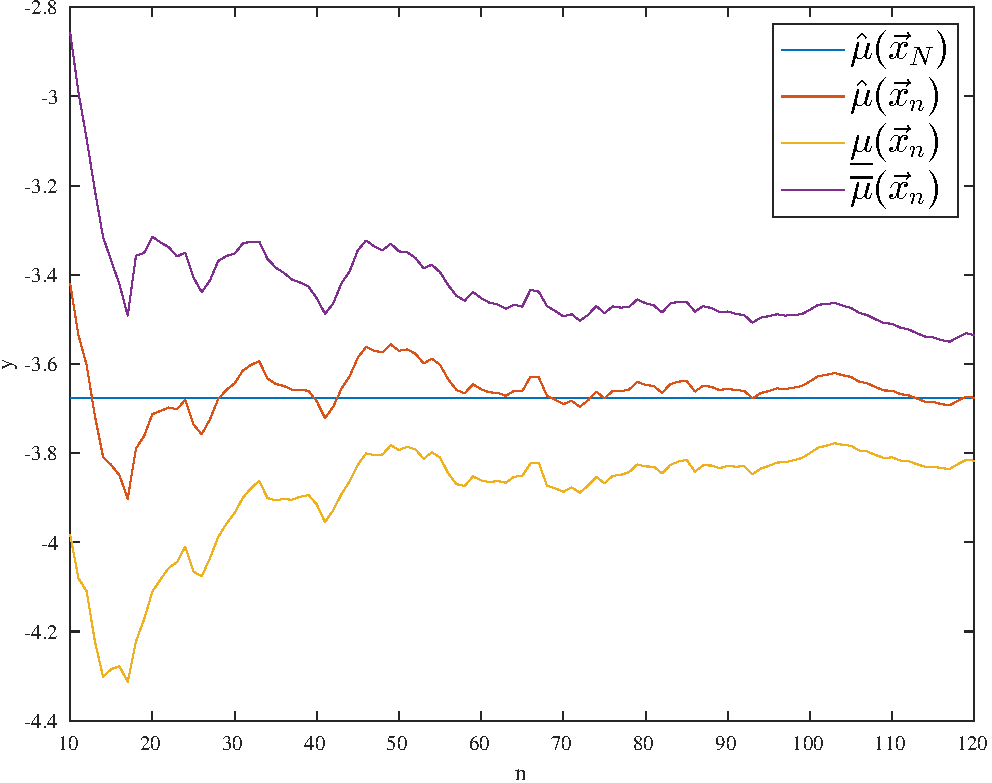
\includegraphics[scale=1]{plots/graph_1_fix.pdf}
    \caption{}
    \label{img:plot01}
\end{figure}

На рисунке \ref{img:plot02} представлены график оценки дисперсии.
\begin{figure}[H]
    \centering
    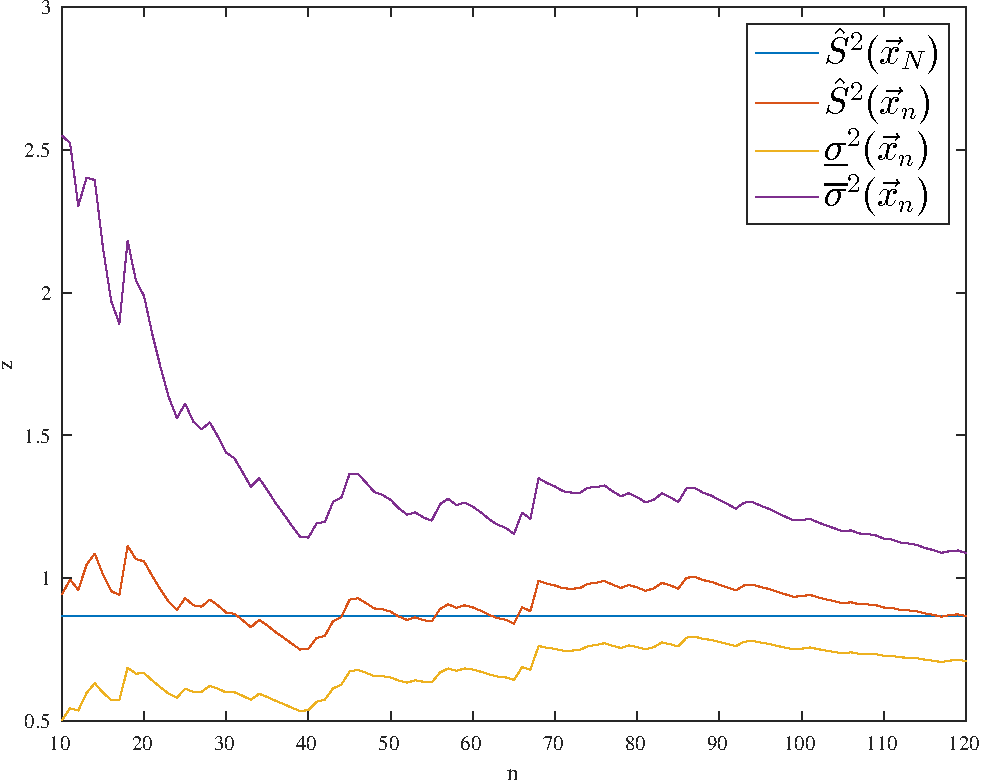
\includegraphics[scale=1]{plots/graph_2_fix.pdf}
    \caption{}
    \label{img:plot02}
\end{figure}

